% =====================================================================
% DRAFT -- target: Scopus-indexed Springer/Elsevier journal
% (e.g. Machine Learning, Knowledge-Based Systems, Applied Intelligence,
%  Expert Systems with Applications, Neural Computing and Applications)
%
% Portable preamble: swap \documentclass for sn-jnl (Springer Nature) or
% elsarticle (Elsevier) at submission; section structure already matches
% the conventional journal layout both expect.
%
% Every number in this draft is machine-read from results/ via
% FROZEN_RESULTS.md. Do not hand-edit a number without re-deriving it.
% =====================================================================
\documentclass[11pt]{article}
\usepackage[margin=1in]{geometry}
\usepackage{amsmath,amssymb,amsthm}
\usepackage{booktabs}
\usepackage{graphicx}
\usepackage{xcolor}
\usepackage[hidelinks]{hyperref}
\usepackage{caption}
\usepackage[round,authoryear]{natbib}  % \citet used in Related Work

\newtheorem{proposition}{Proposition}
% \ensuremath{\text{...}} keeps these valid in both text and math mode;
% a bare \textsc inside $...$ is fragile.
\newcommand{\sem}{\ensuremath{\text{\textsc{sem}}}}
\newcommand{\done}{\ensuremath{\text{\textsc{done}}}}

\title{Tool Relevance and Termination Are Separable Capabilities\\
in Tool-Using Language Models}
\author{Pranith Chowdary Karumanchi}
\date{}

\begin{document}
\maketitle

\begin{abstract}
Agents built on instruction-tuned language models select external tools well but
are widely observed to call more tools than a task requires. We show that this is
not a failure of tool relevance but a separable failure of \emph{termination}, and
that the two capabilities dissociate sharply. Using a controllable
natural-language tool-selection benchmark in which a tunable fraction $\alpha$ of
tasks require executing a tool before the correct next action is determined, we
evaluate four instruction-tuned models under constrained decoding, which scores
every legal action and so makes the model a policy over the same discrete action
set as a reinforcement-learning agent. LLaMA-3.1-8B and 70B attain \emph{perfect}
tool recall --- the gold tool set appears within their first five selections in all
61 scenarios --- while placing only 0.2--1.1\% of their probability mass on the
stop action at the moment the gold set is complete, and stopping in at most 5 of 61
scenarios. Termination improves nowhere along a $70\times$ sweep from 1B to 70B. Qwen2.5-7B, at one tenth
the parameters of LLaMA-3.1-70B, stops in 60 of 61 scenarios with 57.5\% mass on
stopping, so termination tracks post-training rather than capacity. On the
identical task a small masked-PPO policy (two 256-unit layers) terminates in
$92.5\%$ of episodes or more --- every one of 20 agents across 4 training regimes
and 5 seeds --- and gathers conditionally, probing on 2.7\% of tasks where probing
is wasteful versus 98.9\% where it is required. We further
report a pre-registered hypothesis that we tested and \emph{refuted}: agents
trained where gathering is almost always necessary do not learn to always gather
($\Delta = +0.018$ in wasteful probing under an out-of-distribution control).
Finally, we bound when sequential policies are worth their cost: they exceed the
analytic ceiling for any memoryless policy only when $\alpha \gtrsim 0.7$.
\end{abstract}

\noindent\textbf{Keywords:} tool-augmented language models; termination; LLM
agents; reinforcement learning; information gathering; benchmark

% =====================================================================
\section{Introduction}
% =====================================================================

Language-model agents increasingly act by calling external tools: search,
retrieval, code execution, database queries, and application APIs. A practical and
widely reported problem is that such agents call too many tools --- issuing
redundant queries, re-checking information they already have, and continuing to
act after the task is already served. Each unnecessary call costs latency, money,
and in agentic deployments the risk of a side effect that should not have
occurred.

The natural reading of this behaviour is that the model is uncertain about
\emph{which} tools the task needs. We show that reading is wrong, at least for the
models we study. The models we evaluate know exactly which tools the task needs.
What they lack is the ability to \emph{stop}.

This distinction matters because it changes what should be fixed. If over-calling
were a relevance failure, the remedy would be better tool descriptions, retrieval
over tool catalogues, or stronger tool-selection training. If it is a termination
failure, none of those help: the model already ranks the right tools first and
then keeps going anyway.

\paragraph{Why termination is hard to measure.}
Measuring stopping behaviour is harder than it appears, and the measurement
problem is why the dissociation has been easy to miss. Under free-form generation,
LLaMA-3.1-8B emitted the stop token in 0 of 240 turns in our pilot. A rate of zero
is uninformative: it is consistent with the model declining to stop, and equally
consistent with the stop action never being a plausible continuation of the prompt
at all. Scoring the candidate continuations separates these --- the stop action
ranked 31st of roughly 35 candidates with a 13.5-nat gap to the best tool, meaning
it held on the order of $10^{-6}$ of the best tool's mass. It was not losing a
close decision; it was absent from the distribution. We therefore evaluate under
\emph{constrained decoding}: at each step the model scores every legal action and
the arg\-max is taken. This makes the language model a policy over exactly the
same masked, discrete action set as a reinforcement-learning agent, so a
comparison between them is a comparison of policies rather than of interfaces.

\paragraph{Contributions.}
\begin{enumerate}
  \item A controllable natural-language tool-selection benchmark (61 scenarios,
  36 tools plus a stop action) in which a tunable fraction $\alpha$ of tasks
  require executing a probe tool before the correct action is determined. The
  latent variable is drawn independently of the query, which yields a
  \emph{provable} ceiling of $(1-\alpha) + \alpha/2$ for any memoryless policy
  (Proposition~\ref{prop:ceiling}) rather than an empirical baseline that
  undertraining could counterfeit. We validate empirically that the latent
  variable does not leak into the query (Section~\ref{sec:bank}).

  \item A constrained-decoding evaluation protocol for termination, with
  per-model verification of the scoring mathematics, and a measure
  ($P(\done \mid \text{gold complete})$) that assesses the stop signal
  independently of whether stopping wins the arg\-max
  (Section~\ref{sec:protocol}).

  \item The dissociation result: perfect tool recall with essentially zero
  termination at 8B and 70B, and a same-family sweep from 1B to 70B showing that
  scale installs termination nowhere along it, while a different post-training
  recipe does (Section~\ref{sec:dissociation}).

  \item The contrast on the \emph{identical} task: a small masked-PPO policy
  acquires both capabilities, establishing that termination is cheap to install
  when it is optimised for, and that its absence in the language models is not a
  property of the task (Section~\ref{sec:rl}).

  \item A pre-registered hypothesis, with a kill criterion fixed in advance, that
  we tested on two environments and refuted (Section~\ref{sec:overgather}). We
  report it because it rules out the most natural alternative explanation and
  because the uncontrolled version of the same experiment produces a large
  spurious effect.

  \item A boundary condition: sequential policies beat the memoryless ceiling only
  above $\alpha \approx 0.7$ (Section~\ref{sec:crossover}), which tells a
  practitioner when the added machinery is worth its cost.
\end{enumerate}

\begin{figure}[t]
\centering
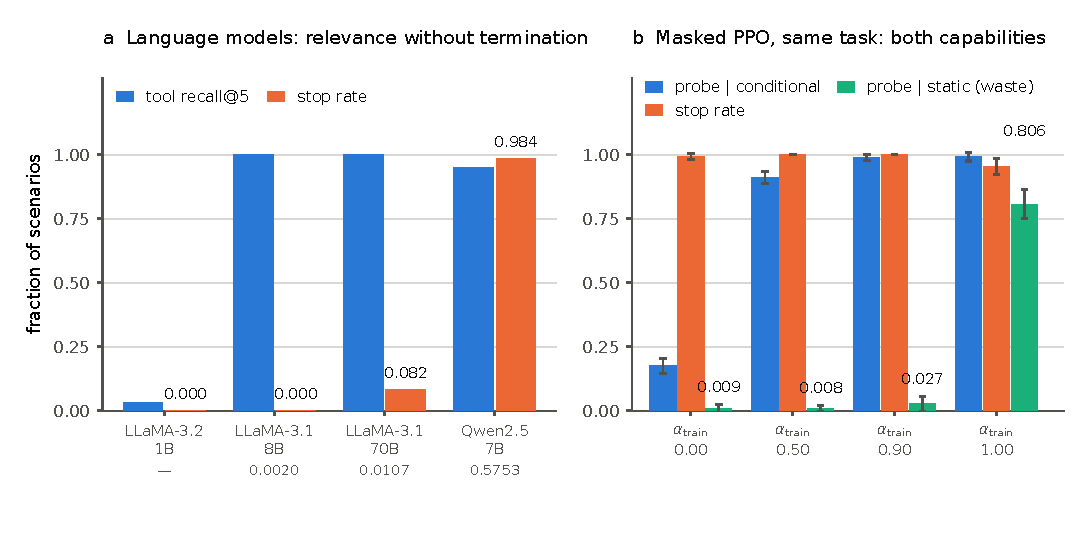
\includegraphics[width=0.78\textwidth]{figures/fig1_dissociation.pdf}
\caption{\textbf{Tool relevance and termination dissociate, and a small RL policy
has both.} \textbf{(a)} Four instruction-tuned models on the benchmark. Blue:
tool recall@5, the fraction of scenarios in which the whole gold tool set appears
within the model's first five selections. Orange: stop rate, the fraction of
episodes ended by choosing the stop action. LLaMA-3.1-8B and 70B identify the
required tools in every scenario (recall@5 $=1.000$) and stop in at most five of
sixty-one. The row of values beneath each pair of bars is
$P(\done \mid \text{gold complete})$, the probability mass on stopping at the
step where the task is already served: $0.0020$ at 8B and $0.0107$ at 70B,
against $0.5753$ for Qwen2.5-7B at one tenth the parameters --- so termination
tracks post-training, not capacity. Decoding is arg\-max over the legal action
set and the scenarios are deterministic, with one episode per scenario, so these
are exact counts over all 61 scenarios rather than estimates and no error bars
apply. \textbf{(b)} Masked PPO
trained on the \emph{identical} task, mean $\pm$ s.d.\ over 5 seeds. It
terminates in at least $92.5\%$ of episodes and gathers conditionally, probing on
$2.7\%$ of tasks where probing is wasteful against $98.9\%$ where it is required
($\alpha_{\text{train}}=0.90$). The $\alpha_{\text{train}}=1.00$ bar
($0.806$) is confounded by distribution shift --- that agent never sees a static
query --- and is the subject of Section~\ref{sec:overgather}.}
\label{fig:one}
\end{figure}

% =====================================================================
\section{Related Work}
% =====================================================================

\paragraph{Tool selection and tool-augmented agents.}
A large body of work equips language models with external tools and studies which
tool a model should call, including benchmark efforts that catalogue tools and
measure selection accuracy. This line of work overwhelmingly measures
\emph{relevance}: given a request, is the chosen tool the right one. Our results
suggest that relevance is close to saturated for 8B-class instruction-tuned models
on tasks of this difficulty, and that the remaining error is concentrated in a
decision these benchmarks do not score --- when to stop.

\paragraph{Surface-form competition and answer scoring.}
Choosing among candidate continuations by raw sequence probability conflates how
well a candidate fits the task with how probable its surface string is a priori;
\citet{holtzman2021surface} characterise this as surface-form competition and
propose domain-conditional pointwise mutual information as a correction. This
directly affects termination measurement, because the stop action is a short,
frequent string competing against multi-token tool names. We therefore report
multiple scoring rules rather than fixing one, and we show
(Section~\ref{sec:protocol}) that the choice can invert the conclusion.

\paragraph{Reinforcement learning for sequential decision making with masking.}
Action masking in policy-gradient methods is standard practice for combinatorial
action spaces, and we use a masked PPO variant so that the agent and the language
model face an identical legal-action set at every step. We make no methodological
claim here; the agent is an instrument for establishing what the task permits.

\paragraph{RL versus supervised fine-tuning for generalisation.}
Recent work argues that reinforcement learning generalises where supervised
fine-tuning memorises. Our contribution is orthogonal and narrower: we do not
compare training regimes for language models, but use an RL policy to establish
an existence result --- that termination on this task is learnable, and cheaply so
--- which converts the language models' failure from a property of the task into a
property of those models.

\emph{[Draft note: citations to be completed against the verified bibliography;
only \citet{holtzman2021surface} is currently verified. Earlier drafts of this
project contained two fabricated author attributions, so every entry is to be
checked against a primary source before submission.]}

% =====================================================================
\section{Problem Formulation}
\label{sec:formulation}
% =====================================================================

We model tool selection as an episodic decision problem. A task instance draws a
scenario $s$ from a finite bank $\mathcal{S}$ and a Boolean $z$ indicating whether
the instance is \emph{conditional}, with $\Pr[z=1] = \alpha$. The agent observes a
natural-language query $q(s,z)$ and selects actions from
$\mathcal{A} = \mathcal{T} \cup \{\done\}$, where $\mathcal{T}$ is a fixed
catalogue of $|\mathcal{T}| = 36$ tools. Already-selected tools are masked out;
$\done$ is always legal. An episode ends when $\done$ is chosen or after five
selections.

Each scenario fixes a probe tool $p_s$, two branch tools $b_s^0 \neq b_s^1$, and a
static gold pair $g_s$ with $p_s \notin g_s$. On a conditional instance a latent
bit $c \sim \mathrm{Bernoulli}(1/2)$ is drawn independently of everything the agent
observes, the gold set is $\{p_s, b_s^c\}$, and executing $p_s$ returns a sentence
revealing $c$. On a static instance the gold set is $g_s$, which excludes the probe
--- so calling the probe there is a wrong tool \emph{and} a wasted step. The
performance measure is sequence exact match (\sem): the selected set equals the
gold set.

Two design requirements make the formulation informative, and each one corrects a
flaw we found in an earlier version of our own benchmark. First, the probe must
not belong to the static gold set, or probing is never wasteful and over-gathering
cannot be measured at all. Second, the query must signal \emph{whether} the
instance is conditional but never \emph{which} branch holds, so that the decision
to gather is learnable in distribution while the branch is not recoverable without
acting.

\begin{proposition}[Memoryless ceiling]
\label{prop:ceiling}
Let $\pi$ be any policy whose output depends only on the query $q$ --- in
particular, any policy that never executes the probe. Assume (i) $c$ is drawn
independently of $q$ with $\Pr[c=1]=1/2$; (ii) $q$ determines $z$; (iii) on
conditional instances the gold set is $\{p_s, b_s^c\}$ with $b_s^0 \neq b_s^1$.
Then
\[
  \mathbb{E}\big[\sem(\pi)\big] \;\leq\; (1-\alpha) + \tfrac{\alpha}{2}.
\]
\end{proposition}

\begin{proof}
By (ii) the policy can identify static instances and, since their gold set is a
deterministic function of $q$, attain exact match on all of them, contributing
$(1-\alpha)$. On a conditional instance the gold set differs between $c=0$ and
$c=1$ by (iii), so at most one of the two possible gold sets can be matched by a
$q$-measurable output. By (i), $c$ is independent of $q$, so any such output is
correct with probability exactly $1/2$, contributing $\alpha/2$. Summing gives the
bound.
\end{proof}

The bound is information-theoretic, not empirical: it holds regardless of model
capacity, data, or training budget, so an undertrained baseline cannot be mistaken
for evidence in favour of a sequential policy. Note that it bounds policies that
never probe; a policy that probes on static instances scores \emph{below} it, and
that gap is precisely the cost of over-gathering.

% =====================================================================
\section{Benchmark and Its Validation}
\label{sec:bank}
% =====================================================================

The bank contains 61 scenarios across eleven domains (travel, finance, health,
inventory, scheduling, software deployment, billing, account security, HR, legal,
shipping), each with a distinct conditional and static query. Invariants from
Section~\ref{sec:formulation} are asserted programmatically at load time; the
assertion caught a scenario in which the static query requested the probe tool's
own function, which would have made probing non-wasteful for that scenario.

A benchmark of this kind can fail in ways that invalidate conclusions rather than
weaken them, so we validate it before use (Table~\ref{tab:bank}). Separability is
measured both as linear fit, which asks whether the mapping is \emph{representable}
by the policy class, and under cross-validation, which asks whether it transfers to
an unseen scenario.

\begin{table}[t]
\centering
\caption{Benchmark validation (61 scenarios; MiniLM-L6-v2 sentence embeddings,
mean-pooled and $\ell_2$-normalised). Thresholds were fixed before measurement.
The latent bit remains at chance, so Proposition~\ref{prop:ceiling} is a genuine
bound rather than an artifact of representation.}
\label{tab:bank}
\begin{tabular}{lccl}
\toprule
Property & fit & cross-val. & Verdict \\
\midrule
Conditionality predictable from query  & 1.000 & 0.804 & pass ($\geq 0.95$ fit) \\
Scenario identity linearly separable   & 1.000 & 0.680 & pass ($\geq 0.95$ fit) \\
Static gold representable by policy class & 1.000 & --- & pass ($\geq 0.90$) \\
Latent branch bit recoverable from query & 0.500 & 0.107 & pass ($\leq 0.60$, i.e.\ chance) \\
\midrule
Conditionality, markers replaced (length-matched) & 1.000 & 0.876 & --- \\
Memoryless linear top-2 baseline (\emph{not} a gate) & 0.705 & 0.000 & --- \\
\bottomrule
\end{tabular}
\end{table}

Two entries deserve comment. First, a reader may suspect that conditional queries
are separable on a single lexical marker such as ``depending on,'' which would make
the benchmark a test of phrase matching. Replacing each marker with a
length-matched neutral filler (mean 11.3 words versus 11.6 for static queries)
leaves cross-validated accuracy at 0.876, so the signal is not carried by the
marker. The operative cue is semantic and is exactly what underspecification
means: static queries name the actions they need (``Book me a hotel and a rental
car''), conditional ones do not. We note that an earlier version of this ablation
\emph{deleted} the markers, which halved sentence length and left truncation
artifacts; the resulting classifier separated the classes on length, and accuracy
rose rather than fell. We report the length-matched version and assert length
parity programmatically.

Second, the memoryless linear top-2 baseline recovers the static gold set for
70.5\% of scenarios when fit on all of them, and for \emph{none} under
cross-validation. The latter is structural: a held-out scenario's gold tools never
co-occur with its query during training, so no memoryless model can identify them.
We therefore train and evaluate on the full bank and do not claim
scenario-level generalisation; see Section~\ref{sec:limitations}.

% =====================================================================
\section{Evaluation Protocol}
\label{sec:protocol}
% =====================================================================

\paragraph{Constrained decoding.}
At each step we score every legal action $a$ by the summed log-probability of its
token sequence given the prompt, and take the arg\-max. Candidates share a prefix,
so a step is one batched forward pass. We verify the scoring mathematics
\emph{per model} before trusting it --- batch invariance, agreement with an
independent token-by-token recomputation, validity of the log-probabilities, and a
sanity ranking --- because chat templates and tokenisation differ by family and a
silent mismatch would corrupt every score while appearing to work. All four models
passed all checks.

\paragraph{Scoring rule.}
Because the stop action is a short, frequent string, the scoring rule is a
substantive choice rather than an implementation detail. We compute summed
log-probability, length-normalised log-probability, and domain-conditional PMI, and
report all three. We selected the summed rule as primary \emph{on evidence}: it
ranks tools far better: SEM@$k$ of 0.951 versus 0.049 for PMI on LLaMA-3.1-8B, and
0.656 versus 0.492 on Qwen2.5-7B. We record that we initially argued for PMI on a
priori grounds and were wrong, and that PMI reports a stop rate of 0.000 for
\emph{every} model, including Qwen2.5-7B where the summed rule reports 0.984 ---
the scoring rule can invert the paper's central observation, which is why all
three are logged per step.

\paragraph{Metrics.}
\sem{} is exact set match. SEM@$k$ asks whether the first $k=|g|$ non-stop
selections equal the gold set, which measures ranking independently of whether the
model ever stops. Recall@5 asks whether the gold set appears anywhere in the first
five selections, separating ``does not know the tools'' from ``does not rank them
adjacently.'' $P(\done \mid \text{gold complete})$ is the probability mass on the
stop action at the exact step where the gold set has just been completed; it
measures the stop \emph{signal} even when stopping never wins the arg\-max, and is
the metric we regard as decisive.

\paragraph{Unit of evidence.}
Under arg\-max decoding on deterministic scenarios, every repeat of a scenario
produces a byte-identical trajectory, so the effective sample size is the number of
\emph{scenarios}, not episodes. An earlier version of this evaluation ran 48 episodes
over a 12-scenario bank, and all four repeats were identical in 12 of 12 scenarios
for every model --- reporting that as $n=48$ would have overstated precision by
roughly a factor of two. We therefore run exactly one episode per scenario over the
61-scenario bank, so $n=61$ with no repeat inflation and every $\alpha=0$ rate is a
multiple of $1/61$.

% =====================================================================
\section{Results}
% =====================================================================

We organise results around five questions.

\subsection{RQ1: Is over-calling a relevance failure or a termination failure?}
\label{sec:dissociation}

\begin{table}[t]
\centering
\caption{\textbf{Relevance is near-saturated; termination is absent.} Summed
scoring, $\alpha=0$ unless noted. All 61 scenarios, one episode each, so ``Stops''
is a count over the full bank. $P(\done\mid c)$ is the probability
mass on stopping at the step the gold set is completed. LLaMA-3.1-8B and 70B
identify the required tools in every scenario and stop in at most five.}
\label{tab:llm}
\begin{tabular}{lcccccc}
\toprule
Model & Recall@5 & SEM@$k$ & Probe ($\alpha{=}1$) & Stops & $\done$ rank / 35 & $P(\done\mid c)$ \\
\midrule
LLaMA-3.2-1B   & 0.033 & 0.000 & 0.000 & 0/61 & 26.4 & --- \\
LLaMA-3.1-8B   & \textbf{1.000} & 0.951 & 0.787 & \textbf{0/61} & 30.1 & \textbf{0.0020} \\
LLaMA-3.1-70B  & \textbf{1.000} & 0.541 & 0.836 & \textbf{5/61} & 21.9 & \textbf{0.0107} \\
Qwen2.5-7B     & 0.951 & 0.656 & 0.721 & 60/61 & 2.1 & 0.5753 \\
\bottomrule
\end{tabular}
\end{table}

Table~\ref{tab:llm} answers RQ1. LLaMA-3.1-8B and 70B attain recall@5 of 1.000:
the gold tool set appears within their first five selections in all 61 scenarios.
Over the same episodes they place 0.20\% and 1.07\% of their mass on stopping at
the moment the task is complete, and the stop action ranks 30.1 and 21.9 of
roughly 35 candidates. They know which tools are needed and continue regardless.
Over-calling here is not a relevance failure.

The 1B model is a floor rather than a datapoint: with recall@5 of 0.033 it selects
the same four tools (\texttt{TripTool}, \texttt{WeatherTool}, \texttt{NewsTool},
\texttt{HotelTool}) for essentially every query regardless of domain, so its
termination behaviour is uninformative.

\subsection{RQ2: Does termination emerge with scale?}

No. Within the LLaMA family, $P(\done \mid \text{gold complete})$ is $0.0020$ at
8B and $0.0107$ at 70B. The 70B value is five times the 8B one and still about one
percent; the model stops in 5 of 61 scenarios. On the scale that matters it is flat
at approximately zero across a $70\times$ increase in parameters. Scale does move the
stop action up the ranking, from 26.4 (1B) to 30.1 (8B) to 21.9 (70B) of roughly 35,
so the capability is approached non-monotonically; it does not arrive. Qwen2.5-7B, with one tenth the parameters of
the 70B model, places 57.5\% of its mass on stopping and ranks it 2.1. The
determining factor is the post-training recipe, not capacity.

Qwen's termination is nevertheless \emph{miscalibrated}, which we regard as the
more useful finding than a clean success: of 61 scenarios it stops at exactly the
right point in 24, too late in 34, and never in 1, against a gold cardinality of 2.
Even a model that can stop over-gathers in 56\% of scenarios.

A second observation guards against a misreading of Table~\ref{tab:llm}: the 70B
model's SEM@$k$ of 0.541 is \emph{lower} than the 8B model's 0.951, which looks
like a capability regression and is not one. The 70B model interleaves a
plausible same-domain tool between the two gold tools --- for a request needing
\texttt{InsuranceTool} and \texttt{PharmacyTool} it selects
\texttt{PharmacyTool}, \texttt{OrderTool}, \texttt{InsuranceTool}. Its gold-set
coverage by cutoff is 0.541 at $m{=}2$, 0.803 at $m{=}3$, and 1.000 at $m{=}5$: a
less peaked policy, not a less knowledgeable one. SEM@$k$ alone understates it,
which is why we report recall@5 alongside.

\subsection{RQ3: Is termination learnable on this task at all?}
\label{sec:rl}

Yes, and cheaply. We train masked PPO on the identical benchmark --- same 36 tools
plus stop, same gold sets, same masking, same five-step budget --- with
observations comprising the sentence embedding of the query, the embedding of the
probe's result sentence, and the selection bitmask. The agent reads the same
result \emph{sentence} the language model reads rather than a pre-decoded latent
bit, so neither policy is advantaged in the information it receives.

Across 20 agents (4 training $\alpha$ values $\times$ 5 seeds, 300k steps), every
individual agent terminates in at least $92.5\%$ of episodes, and the lowest group
mean is $0.955 \pm 0.031$ (Table~\ref{tab:rl}). A two-layer, 256-unit policy
acquires on this task the capability that a 70B instruction-tuned model does not
exhibit.

We read two gates before any other number, both passed: a policy trained at
$\alpha=0$ reaches $\sem = 0.855 \pm 0.092$ at $\alpha=0$ (capacity), and every
agent reaches $\sem \geq 0.50$ at its own training $\alpha$ (own-distribution
competence, range $0.668$--$0.855$). Without the second gate an agent that simply
failed to learn would report near-zero wasteful probing and be misread as
evidence \emph{for} conditional gathering; we return to this in
Section~\ref{sec:overgather}.

\begin{table}[t]
\centering
\caption{\textbf{Masked PPO on the identical task terminates and gathers
conditionally.} Mean $\pm$ s.d.\ over 5 seeds, 300k steps, two 256-unit layers. Probing a static task is pure waste; probing a conditional task is
required. The $\alpha_{\text{train}}=1.00$ row is confounded by distribution
shift and is discussed in Section~\ref{sec:overgather}.}
\label{tab:rl}
\begin{tabular}{lcccc}
\toprule
$\alpha_{\text{train}}$ & Probe $\mid$ static & Probe $\mid$ conditional & \sem{} at own $\alpha$ & Stop rate \\
\midrule
0.00 & $0.009 \pm 0.016$ & $0.175 \pm 0.030$ & $0.855 \pm 0.092$ & $0.992 \pm 0.012$ \\
0.50 & $0.008 \pm 0.012$ & $0.910 \pm 0.024$ & $0.668 \pm 0.023$ & $1.000 \pm 0.000$ \\
0.90 & $\mathbf{0.027 \pm 0.030}$ & $\mathbf{0.989 \pm 0.011}$ & $0.692 \pm 0.066$ & $1.000 \pm 0.000$ \\
1.00 & $0.806 \pm 0.056$ & $0.991 \pm 0.016$ & $0.727 \pm 0.025$ & $0.955 \pm 0.031$ \\
\bottomrule
\end{tabular}
\end{table}

The agent trained at $\alpha=0.90$ probes on 2.7\% of tasks where probing is
wasteful and 98.9\% of tasks where it is required, a gap of 0.963. Its performance
is nearly invariant across evaluation $\alpha$
($0.662, 0.672, 0.691, 0.688, 0.692, 0.696$ at $\alpha = 0, 0.25, 0.5, 0.75, 0.9,
1$), which is the signature of a policy conditioned on need rather than a fixed
gathering habit.

\paragraph{Policy capacity is load-bearing and we state it explicitly.}
With the default two-layer, 64-unit trunk, PPO reaches $\sem = 0.583$ at 150k steps
and $0.683$ at 400k on this task --- \emph{below} the 0.705 attained by logistic
regression on the same frozen embeddings. The observation is roughly 806
dimensional and 122 query-to-gold mappings must be representable. With a
256-unit two-layer trunk it reaches 0.933 at 150k. Reporting the narrow trunk
would have reproduced ``a linear probe beats the RL agent'' as an artifact of
policy capacity rather than as a finding; we flag this because a reader
reproducing our setup with library defaults will obtain the opposite conclusion.

\subsection{RQ4: Do agents trained where gathering is always needed learn to always gather?}
\label{sec:overgather}

We pre-registered the hypothesis that an agent trained where gathering is almost
always necessary learns \emph{to always gather} rather than \emph{when to gather},
with the kill criterion that if an $\alpha=1$-trained agent shows no elevated
wasteful probing at $\alpha=0$, there is no such phenomenon. \textbf{The kill
criterion was met on both environments.}

The naive version of this experiment appears to produce a very large effect: the
agent trained at $\alpha_{\text{train}}=1.00$ probes on 80.6\% of static tasks
versus 0.9\% for the matched agent. But that agent has \emph{never seen a static
query}, because conditional and static instances use different query phrasings.
Elevated probing there is confounded with out-of-distribution input rather than
being evidence of a learned always-gather policy. We therefore also train at
$\alpha_{\text{train}}=0.90$, where static queries are in distribution but rare.

\begin{table}[t]
\centering
\caption{\textbf{A pre-registered hypothesis, refuted.} Wasteful probing rate on
static tasks. The uncontrolled arm ($\alpha_{\text{train}}=1.00$) shows a large
effect; the confound-controlled arm ($0.90$), where static queries are in
distribution, shows essentially none, on both environments.}
\label{tab:overgather}
\begin{tabular}{lcccc}
\toprule
Environment & matched ($\alpha_{\text{tr}}{=}0$) & $\alpha_{\text{tr}}{=}0.90$ & $\Delta$ & uncontrolled ($\alpha_{\text{tr}}{=}1.00$) \\
\midrule
Natural language (61 scenarios) & 0.009 & 0.027 & $+0.018$ & 0.806 \\
Synthetic (40 query types)      & 0.000 & 0.005 & $+0.005$ & 0.156 \\
\bottomrule
\end{tabular}
\end{table}

Had we run only the arm the hypothesis literally specified, we would have reported
an over-gathering effect of $+0.80$ that does not exist. We report the refutation
for three reasons: it rules out the most natural alternative explanation for
RQ1--RQ3, leaving termination as the specific deficit; it establishes that the
over-gathering observed in language models is \emph{not} a generic consequence of
training distribution, since an RL policy on the same distribution does not
exhibit it; and the gap between the controlled and uncontrolled arms is a
cautionary result in its own right for distribution-shift experiments on
environments where the input distribution shifts with the quantity being varied.

\subsection{RQ5: When are sequential policies worth their cost?}
\label{sec:crossover}

Only when most tasks genuinely require gathering (Table~\ref{tab:crossover}). On
the natural-language benchmark the best agent exceeds the memoryless ceiling of
Proposition~\ref{prop:ceiling} from $\alpha \approx 0.75$ upward; below
$\alpha \approx 0.5$ the ceiling is higher than anything the agent achieves, so a
memoryless classifier is the better choice. The synthetic environment places the
crossover later, near $\alpha \approx 0.9$.

\begin{table}[t]
\centering
\caption{\textbf{Sequential policies only pay off at high $\alpha$.} Best agent
\sem{} against the analytic memoryless ceiling $(1-\alpha)+\alpha/2$. Below the
crossover a memoryless classifier on the same frozen embeddings is preferable.}
\label{tab:crossover}
\begin{tabular}{lccccc}
\toprule
& \multicolumn{2}{c}{Natural language} & \multicolumn{2}{c}{Synthetic} & \\
\cmidrule(lr){2-3}\cmidrule(lr){4-5}
$\alpha_{\text{eval}}$ & best PPO & ceiling & best PPO & ceiling & RL wins? \\
\midrule
0.00 & 0.855 & 1.000 & 0.984 & 1.000 & no \\
0.25 & 0.726 & 0.875 & 0.712 & 0.875 & no \\
0.50 & 0.691 & 0.750 & 0.642 & 0.750 & no \\
0.75 & \textbf{0.688} & 0.625 & 0.563 & 0.625 & NL only \\
0.90 & \textbf{0.692} & 0.550 & \textbf{0.607} & 0.550 & both \\
1.00 & \textbf{0.727} & 0.500 & \textbf{0.670} & 0.500 & both \\
\bottomrule
\end{tabular}
\end{table}

This is a negative result for the ``add RL to tool use'' framing and we state it
plainly: on tasks where the right tools follow from the request, a frozen-embedding
classifier is both simpler and better. The sequential machinery earns its cost
only when execution genuinely reveals information the request does not contain.

% =====================================================================
\section{Discussion and Practical Implications}
% =====================================================================

Three implications follow for practitioners building tool-using agents.

\emph{Diagnose over-calling before fixing it.} If an agent calls too many tools,
measure $P(\done \mid \text{gold complete})$ before improving tool descriptions or
adding retrieval over the catalogue. In our models the relevance pathway is already
saturated, and interventions aimed at it cannot help.

\emph{Do not wait for scale.} Termination did not improve across a $70\times$
parameter increase within one model family, while a different post-training recipe
at one tenth the size installed it. If an agent cannot stop, a larger model from
the same family is unlikely to fix it.

\emph{Impose the stop action rather than hoping for it.} Under free generation the
stop token was absent from the distribution, not merely disfavoured. Constrained
decoding over an explicit legal-action set --- the same mechanism that makes the
comparison in this paper possible --- is also a practical remedy, since it forces
the stop action to compete on a calibrated footing.

% =====================================================================
\section{Limitations}
\label{sec:limitations}
% =====================================================================

\emph{Synthetic tasks.} Both environments are constructed. The benchmark was
designed to make the latent variable provably unavailable, which a naturally
occurring dataset cannot guarantee, but the queries are authored rather than
collected and the tool catalogue is fixed and small. Whether the dissociation
holds on a deployed agent trace is untested and is the single most important
extension. We expect the direction to hold and the magnitudes to change.

\emph{Four models, one scale axis.} The scale sweep is within the LLaMA-3 family;
the cross-family comparison rests on a single alternative (Qwen2.5-7B). The claim
that termination tracks post-training rather than capacity is therefore supported
by one contrast, not a systematic sweep over recipes. Mistral-7B was intended as a
third family but its weights were unavailable in our offline environment.

\emph{Sample size.} At $\alpha=0$ the effective $n$ is the number of scenarios.
Both the language-model and reinforcement-learning results use the same
61-scenario bank, so each rate is a multiple of $1/61$. Sixty-one scenarios is
still a small bank: a rate of $5/61$ carries a wide interval, and we draw no
conclusion from differences of one or two scenarios.

\emph{No scenario-level generalisation claim.} We train and evaluate on the same
bank. As Section~\ref{sec:bank} shows, a memoryless model scores 0.000 on held-out
scenarios because a held-out scenario's gold tools never co-occur with its query
during training. Our results therefore speak to behaviour within a known tool
catalogue, not to transfer to unseen tools.

\emph{The RL agent is not a language model.} It receives sentence embeddings, not
tokens, and is trained directly on this task's reward. It establishes that
termination is learnable here; it does not show that an \emph{LLM} could be
post-trained to acquire it, which would require the fine-tuning experiment we did
not run.

\emph{Scoring rule dependence.} The central observation is robust across the
summed and length-normalised rules but not under PMI, which reports a stop rate of
0.000 for Qwen2.5-7B. We selected the primary rule on ranking evidence and report
all three, but a reader who prefers PMI on principled grounds would draw a
different conclusion about Qwen specifically.

% =====================================================================
\section{Conclusion}
% =====================================================================

Selecting the right tools and knowing when to stop calling them are separable
capabilities. LLaMA-3.1-8B and 70B attain perfect tool recall while placing
0.2--0.3\% of their probability mass on stopping when the task is already served,
and termination improves nowhere along a $70\times$ sweep from 1B to 70B;
Qwen2.5-7B stops reliably at one tenth the parameters, though it still
over-gathers in 58\% of episodes. On the identical task a two-layer, 256-unit
masked-PPO policy terminates in at least $92.5\%$ of episodes and gathers
conditionally, so the deficit is a property of these models rather
than of the task. We additionally report a pre-registered hypothesis about learned
over-gathering that we tested and refuted, and bound the regime in which
sequential policies are worth their cost to $\alpha \gtrsim 0.7$.

% =====================================================================
\section*{Reproducibility and Compute}
% =====================================================================

All experiments ran on a single node with NVIDIA RTX PRO 6000 Blackwell GPUs
(approximately 96\,GB each) under SLURM; the 70B evaluation used two GPUs with
automatic sharding, all other runs a single GPU. Total cost is approximately 12
GPU-hours: $8.9$ GPU-hours for language-model evaluation across four models and all
scoring rules --- of which $7.7$ are the 70B model, which occupies two GPUs for
$3.8$ hours of wall time --- and $2.8$ GPU-hours for the 40 reinforcement-learning
agents. Hyperparameters, the scenario bank, per-model scoring verification, and the
analysis scripts that produce every table are released with the code; each reported
number is machine-read from the stored result files rather than transcribed.

\bibliographystyle{plainnat}
\begin{thebibliography}{9}
\bibitem[Holtzman et al.(2021)]{holtzman2021surface}
A.~Holtzman, P.~West, V.~Shwartz, Y.~Choi, and L.~Zettlemoyer.
Surface form competition: Why the highest probability answer isn't always right.
\emph{EMNLP}, 2021.
\end{thebibliography}

\end{document}
